%Oppgave 2: Innovasjon og mennesker 


\subsection{Oppgave A}
Vi vil her vurdere kvaliteten på jobbene til sveiser og økonomisjef i Tungesvik Stålesveis i henhold til de fem hovedelementene som, i følge jobbkarakteristikamodellen, påvirker en arbeidstakers indre motivasjon.

\subsubsection{Sveiserne}
I produksjonsavdelingen, hvor sveiserne jobber, er arbeidet delt inn i små arbeidsoppgaver.
Den enkelte arbeider er ekspert på spesielle arbeidsoppgaver.
Dermed er graden av ferdighetsvariasjon er liten.
I et intervju git en sveiser uttrykk for frustrasjon over lite variasjon av arbeidsoppgaver.
Vedkommende sier at “Vi er gått over fra å være håndverkere til å bli fabrikkarbeidere”.

Under produksjon av individuelle deler har sveiserne lav oppgaveidentitet.
En sveiser gjør kun en liten del av produksjonen, og ser ikke helheten da vedkommende ikke deltar i alle fasene til produktet han bygger.
De sveiserne som får være med ut til kunden for å gjøre sluttmontering har høyere oppgaveidentitet enn de som ikke får være med der.
Dette underbygges av en uttalelse om at “Sluttmonteringa er mest spennende, for da ser vi helheten i det vi ellers gjør”.

Sveisernes oppgaveviktighet er også forholdsvis lav.
Hvis en sveiser ikke gjør jobben sin, vil det ha betydning for kvaliteten av produktet.
Dette kan i verste konsekvens bety at jobben må gjøres om igjen.

Sveiserne må forholde seg til strenge retningslinjer, og de kan i liten grad bestemme hvordan de skal utføre arbeidet sitt.
Liten frihet til å planlegge arbeidet sitt resulterer i lav autonomi, og dette påvirker arbeidstakerens indre motivasjon negativt.
Denne påstanden underbygges av utsagnet til den ene sveiseren hvor vedkommende sa at de har gått fra å være håndtverkere til å bli fabrikkarbeidere.

I enkelte tilfeller hvor et produkt har en feil på seg, vil man kunne spore opphavet tilbake til sveiseren.
Dette forutsetter at feilen oppdages før produktet er ute hos kunden.
En sveitser har dermed begrenset feedback.

\subsubsection{Økonomisjef}
Når det gjelder Helle Loholt, så har nok hun en høyere score på ferdighetsvariasjon enn sveiserne. Hun er økonomisjef, og trenger å bruke hele sin brede kunnskap om hvordan en bedrift fungerer med tanke på avtaler, hvordan det er lurt å bruke penger, offentlige krav til rapporter og skjemaer, og så videre.

Helle har også høy oppgaveidentitet. Hun har hatt ansvaret for bedriftsøkonomien i hele omstillingsprosessen til bedriften, og ser helheten av det hun gjør. Hun er med på alt arbeidet som gjøres innen økonomi, bortsett fra at hun får hjelp av kontordame og arkivar Marit Nymo.

Oppgaveviktigheten til Helle er også høyere enn sveisernes. Denne stillingen går ut på å balansere budsjettet og holde orden i økonomien til bedriften. Hvis det slurves i denne jobben, kan det bety at hele bedriften går konkurs, og da mister alle i bedriften jobben.

Økonomisjefen har i mye større grad enn sveiserne frihet til å planlegge arbeidet slik hun ønsker, og hun har derfor høyere autonomi. Hun har selv tatt initiativet til arbeid som resulterte i gode finansieringsavtaler for bedriften, noe som viser at hun er selvstendig i arbeidet sitt som økonomisjef.

Økonomisjefen får også tilbakemelding i høyere grad enn sveiserne, da hun ganske konkret får informasjon om arbeidet hennes gjennom firmaets fortjeneste. Man vil kunne se resultatet av hennes finansieringsavtaler og hvordan dette påvirker bedriftens økonomi direkte. Det kan på en annen side ta tid før hun får tilbakemelding på hennes beslutninger, noe som vil trekke ned.

\subsubsection{Motivasjonspotensiale}
\begin{figure}[ht!]
    \centering
    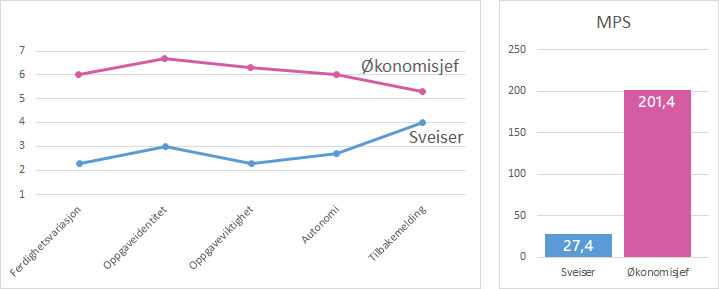
\includegraphics[width=135mm]{mps.png}
    \label{fig:mps}
\end{figure}
I figur \ref{fig:mps} ser vi en grov vurdering av motivasjonspotensialet til en sveiser og en økonomisjef i selskapet, basert på Hackman and Oldman’s Job Diagnostic Survey. Som vi ser, har økonomisjefen en mye høyere MPS (motivating potential score) enn sveiseren.


\subsection{Oppgave B}
\subsubsection{Forslag til tiltak}
Vi vurderer jobbsituasjonen til økonomisjef Helle som god, men sveisernes jobber har forbedringspotensiale. Her kommer noen forslag til tiltak som kan øke sveisernes indre motivasjon, ytelse og jobbtilfredshet:

\begin{itemize}
  \item Ruller arbeidsoppgaver og la alle få delta på sluttmontering. Dette kan føre til høyere ferdighetsvariasjon, oppgaveidentitet, autonomi og tilbakemelding. Kort sagt får de brukt flere ferdigheter, får være med å bestemme hvordan ting blir gjort, de ser helheten av produktet og de kan få tilbakemelding om produktet fra kunden i sanntid.
  \item Flere besøk og samtaler mellom produksjonsavdelingen og ledelsen. La sveiserne ha regelmessige, korte møter med tegneren av maskinene som produseres. Da kan de føle at de får være med mer i diskusjonen av hvordan maskinene designes. De får altså mer oppgaveidentitet og autonomi.
\end{itemize}

Negative konsekvenser av forslagene kan f.eks. være at mer rullering kan føre til mindre ekspertise på spesielle arbeidsoppgaver. Flere møter, besøk og samtaler kan føre til at mindre tid blir brukt på produksjon. Totalt sett kan dette føre til lavere kvalitet og effektivitet.

